\documentclass{article}

%----------------------------------------
% Packages
%----------------------------------------
\usepackage[left=1in, right=1in, top=1in, bottom=1in]{geometry}
\usepackage{graphicx}
\usepackage{amsmath,amsbsy,amssymb,amsfonts,amsthm}
\usepackage{nicefrac}
\usepackage{mathtools}
\usepackage{color}
\usepackage{xspace} % Correct macro spacing
\usepackage[numbers]{natbib} % For citations
\usepackage{times}
\usepackage{graphicx,subfigure}
%\usepackage[small,bf]{caption}
\usepackage{algorithm,algorithmic} 
\usepackage{hyperref}
\usepackage[utf8]{inputenc}

\usepackage{tikz}
% Optional PGF libraries
\usetikzlibrary{shapes,snakes}
\usepackage{pgf}
\usepackage{pgflibraryarrows}
\usepackage{pgflibrarysnakes}
\usetikzlibrary{decorations.text}
\usepgfmodule{shapes}
%\usetikzlibrary{arrows}
\usetikzlibrary{decorations.pathmorphing}
\usetikzlibrary{decorations.markings}
\usetikzlibrary{patterns}
\usetikzlibrary{automata}
\usetikzlibrary{positioning}
\usetikzlibrary{calc}
%\usepackage{tikz-cd}
\usepackage{pgfplots}
%\usepackage{tkz-euclide}
%\usetkzobj{all}
\usetikzlibrary{backgrounds}
%\usetikzlibrary{fillbetween,backgrounds}

% Packages to help figure display 
\usepackage{caption}
\usepackage{float}
\usepackage[export]{adjustbox}
% % %

\usepackage{xcolor}
\usepackage{shadethm}

\usepackage{fancyhdr}
\pagestyle{fancy}
\lhead{This is my name}
\rhead{this is page \thepage}

\usepackage{fancyhdr}
\pagestyle{fancy}
\lhead{IFT 6085 - Theoretical principles for deep learning}
\rhead{Lecture 8: February 01, 2018}


\newshadetheorem{thm}{Theorem}
\newshadetheorem{defn}[thm]{Definition}
\newshadetheorem{assm}[thm]{Assumption}
\newshadetheorem{prop}[thm]{Property}
\newshadetheorem{eg}[thm]{Example}

\definecolor{shadethmcolor}{HTML}{F0F0F0}
%\definecolor{shadethmcolor}{HTML}{EDEDED}
%\definecolor{shadethmcolor}{HTML}{EDF8FF}
%\definecolor{shaderulecolor}{HTML}{EDF8FF}
%\definecolor{shaderulecolor}{HTML}{45CFFF}
\setlength{\shadeboxrule}{.4pt}


\setlength\parindent{0pt}

% Packages hyperref and algorithmic misbehave sometimes.  We can fix
% this with the following command.
\newcommand{\theHalgorithm}{\arabic{algorithm}}

%----------------------------------------
% Standard macros
%----------------------------------------


%----------------------------------------
% Project-specific macros
%----------------------------------------

%----------------------------------------
% Header
%----------------------------------------
\title{IFT 6085 - Lecture 8 \\ 
Statistical learning theory: PAC-Bayes bounds}
\date{}

%----------------------------------------
% Document
%----------------------------------------
\begin{document} 

%----------------------------------------
% Abstract
%----------------------------------------
\maketitle
\textbf{Scribes}\hfill
\textbf{Instructor:} Ioannis Mitliagkas\\
\textbf{Winter 2020:} Howard Huang\\
\textbf{Winter 2019:} Zafarali Ahmed, Nadeem Ward\\
\textbf{Winter 2018:} Jérémy Trudel, Lluís Castrejón
\hfill


%----------------------------------------
% Body
%----------------------------------------

\newcommand{\infgc}{\inf_{g \in \mathcal{C}}}
\newcommand{\supgc}{\sup_{g \in \mathcal{C}}}

\newcommand{\Prob}{\mathbb{P}}
\newcommand{\E}{\mathbb{E}}
\newcommand{\reals}{\mathbb{R}}


\section{Summary}
In the previous lecture we introduced the basics of Statistical Learning Theory. We established the setting for PAC Learning and defined the concepts of \textit{risk}, \textit{empirical risk} and \textit{generalization gap}. We then used \textit{Hoeffding's Inequality} to establish a bound on the generalization gap for finite hypothesis classes $\mathcal{H}$.

\vspace{2ex}

In this lecture we continue our crash course on Statistical Learning Theory by introducing new concepts in order to get tighter bounds on the generalization gap, namely \textit{Occam's (Razor) Bound} and \textit{PAC Bayesian learning}. 

\section{PAC Learning}
In this section we recap our notation from last time. Probably Approximate Correct (PAC) Learning is a framework for analyzing machine learning algorithms. Assume that we have a hypothesis class $\mathcal{H}$ - the set of all possible model configurations - and a set of samples that form our dataset $S = \{z_1, z_2, ..., z_n\}$ with $z_i = (x_i, y_i)$ and $z_i \sim \mathcal{D}$ i.i.d - where $\mathcal{D}$ is the data distribution. Assume also that we have defined a bounded function $l: \mathcal{Y} \times \mathcal{Y} \rightarrow [0, 1]$ (loss function) that quantifies the mismatch between two elements of $\mathcal{Y}$. In this PAC Learning setting, we define the performance of a hypothesis using:
\begin{defn}[Risk]
\[
	R[h] = \mathbb{E}_{(x, y) \sim \mathcal{D}}[l(h(x), y)]
\]
\label{true_risk}
\end{defn}
Recall that we do not have access to the data generating procedure, $\mathcal{D}$, so we resort to using the empirical risk evaluated on our data set, $S$:
\begin{defn}[Empirical Risk]
\[
	\hat{R}_s[h] = \frac{1}{n}\sum_{i=1}^{n} l(h(x_i), y_i) = \frac{1}{n}\sum_{i=1}^{n} l(h,z_i)
\]
\end{defn}
Since we can only use $S$ to discover hypotheses, $h_s$, we define a generalization gap based on how well $h_s$ does on the true risk (Equation~\ref{true_risk}):
\begin{defn}[Generalization Gap]
\[
	\epsilon_{gen}(h_s) = | R[h_s] - \hat{R_s}[h_s] |
\]
\end{defn}
Our main result gave us a bound on the sample size:
% In the last lecture using the Hoeffding bound, we obtained the following bound for the generalization error:
% \begin{thm}
% For all $h \in \mathcal{H}$, if 
% \[
%   n = O\left(\frac{log(\frac{1}{\delta})}{\epsilon^2}\right)
% \]
% then 
% \[
% |R[h]-\hat{R}_s[h]|<\epsilon
% \]
% with probability $\geq 1 - \delta$
% \end{thm}

% Note: to obtain this bound we have assumed that $\mathcal{H}$ is countable and finite. 

% This bound is for a specific $h$, but how can we guarantee that all $h_i \in \mathcal{H}$ would have "good" generalization? Motivated by this, we find a bound for all $h_i$ as follows. 

% We start by assuming we have a uniform probability distribution over $\mathcal[H]$: 
% \[
% 	\delta(h) = \frac{\delta}{|\mathcal{H}|}
% \]
% Observe that: 
% \[
% 	\sum_{h \in \mathcal{H}} \delta(h) = \delta \sum_{1}^{|\mathcal{H}|}\frac{1}{|\mathcal{H}|} = \delta
% \]

\begin{thm} For all $h \in \mathcal{H}$, If
\[
	n=\Omega\left(\frac{log(\frac{|\mathcal{H}|}{\delta})}{\epsilon^2}\right)
\]
then with probability at least $1-\delta$:
\[
\big|R[h]-\hat{R}_S[h] \big|<\epsilon
\]
\end{thm}

% Now we show an example on how to compute $|\mathcal{H}|$. We define the \textit{perceptron} class of models as:
% \[
% l(w^Tx+b), w\in \mathbb{R}^d, b\in \mathbb{R}
% \]

% To represent this model, assuming we use 32 bit floats for each learnable parameter, we need \(32(d+1)\) bits, so:
% \[
% |H|=2^{32(d+1)}
% \]\[
% log|H|=log(2^{32(d+1)})
% \]\[
% log|H|=(d+1)log(2^32)
% \]

%%% OCCAM'S RAZOR BOUND %%%

Recall that to get this result we bounded $P \big( \big|R[h_s]-\hat{R}_S[h_s] \big|>\epsilon \big)$ by $P \big( \bigcup_{h \in \mathcal{H}} \big|R[h]-\hat{R}_s[h] \big|>\epsilon \big)$. 
The reason why we couldn't just apply \textit{Hoeffding's inequality} directly on $P \big( \big|R[h_s]-\hat{R}_S[h_s] \big|>\epsilon \big)$ is because the term $\hat{R}_S[h_s]$ is \textbf{not} the average of i.i.d random variables. If we look closely at the term  $$\hat{R}_S[h_s] = \frac{1}{n} \sum_{\forall z \in S} l(h_s,z) $$
$h_s$ is constructed based on the data $z \in S$. These same $z \in S$ are used in the selection of $h_s$ and used again in the losses $l(h_s,z) \; \forall z \in S$ making them dependent. When we consider $h$ to be arbitrarly chosen, then $\hat{R}_S[h]$ doesn't suffer from the dependence problem which makes it an average of independent random variables.


\section{Occam's (Razor) bound } 

Simply put, \emph{Occam's bound} tells us to put a distribution over the countably infinite hypothesis class $\mathcal{H}$ that is independent of dataset $S$ we will receive (The PAC bound can be treated as Occam's bound with a uniform prior).
This can be thought of as ``placing our bets" on the different hypotheses $h \in \mathcal{H}$ prior to seeing the actual data.
We call this distribution the \textit{prior} $P$ on the hypothesis class $\mathcal{H}$. We will see that in doing so we will get bounds on the generalization gap that no longer depend on the size of the hypothesis class, $|\mathcal{H}|$. These bounds now become variable depending on how we weigh each individual hypothesis $h$, i.e. $P(h)$.

This analysis will use the assumption that $\mathcal{H}$ is discrete (countable) in order to use the union bound. Also, we will assume that the loss function $l(h,z)$ is bounded in order to use Hoeffding's inequality. Without loss of generality assume it's bounded on the interval $[0,1]$.


%Simply put, an \emph{Occam's bound} states that if two hypotheses explain the data equally well, the one that makes less assumptions is generally preferable. In this context, we'll use it to state that the generalization loss is near training loss when the number of bits needed to write the rule is small compared to the sample size \cite{pac-bayes}. For the assumption to hold true, we consider that
%$\mathcal{H}$ is finite and we define the following:

%\begin{defn}
%\[
%\epsilon(h)=\sqrt[]{\frac{\log\frac{1}{P(h)}+\log\frac{2}{\delta}}{2n}}
%\]
%\end{defn}

%\begin{defn}
%\[
%\sum_{h\in \mathcal{H}} P(h)=1
%\]
%\end{defn}

\begin{thm} (\citet{pac-bayes})
Given a prior distribution P on $\mathcal{H}$, \(\sum_{\forall h} P(h)=1\), with probability at least \(\geq 1-\delta\) over $S \sim \mathcal{D}^n$ we have that the following holds true for all h $\in \mathcal{H}$:

\[
 R[h]\leq \hat{R}_S[h]+\sqrt[]{\frac{\log\frac{1}{P(h)}+\log\frac{2}{\delta}}{2n}}
\]
\end{thm}

\begin{proof}
This proof follows the same outline as the one seen for PAC learning. For an arbitrary hypothesis $h$ we demand that: 
\[
\mathbb{P}_{S\sim D}(|\hat{R}_s[h]-R[h]| > \epsilon)\leq \delta P(h)
\]
Recall that, by Hoeffding's inequality, we have that: 
\[
\mathbb{P}_{S\sim D}(|\hat{R}_s[h]-R[h]| > \epsilon)\leq 2e^{ -n\epsilon^2}
\]
we can solve for $\epsilon$ by solving $2e^{ -n\epsilon^2} = \delta P(h) $ and obtain $\epsilon(h) = \sqrt[]{\frac{\log\frac{1}{P(h)}+\log\frac{2}{\delta}}{2n}}$.\\

Given this, we can proceed to bounding our hypothesis of interest, $h_S$:
\begin{align*}
\mathbb{P}_{S\sim D}(|\hat{R}_s[h_S]-R[h_S]| > \epsilon(h)) & \leq \mathbb{P}_{S\sim D}\big(\bigcup_{\forall h}|\hat{R}_s[h]-R[h]| > \epsilon \big) \\ 
& \leq \sum_{\forall h} \mathbb{P}_{S\sim D}(|\hat{R}_s[h]-R[h]| > \epsilon) \\
& \leq \sum_{\forall h} \delta P(h) = \delta
\end{align*}
We used the union of all the hypothesis $h$ to  bound our hypothesis of interest $h_S$. line 2 follows from the union bound. 
What this tells us is that with probability at least $1-\delta$ we have: $$|\hat{R}_s[h_S]-R[h_S]| \leq \sqrt[]{\frac{\log\frac{1}{P(h_s)}+\log\frac{2}{\delta}}{2n}}$$
\end{proof}

Notice that this bound is no longer dependent on $|\mathcal{H}|$ and instead has the term $\log \frac{1}{P(h)}$. If our prior distribution gives more probability to $h$ than this term will decrease therefore giving a tighter bound and vise versa. If, however, we don't give any probability to a hypothesis $h$ (i.e $P(h) = 0$) then $\log \frac{1}{P(h)}$ will be undefined which provides a vacuous bound.

\vspace*{0.5cm}
\begin{figure}[H]
    \captionsetup{justification=centering}
	%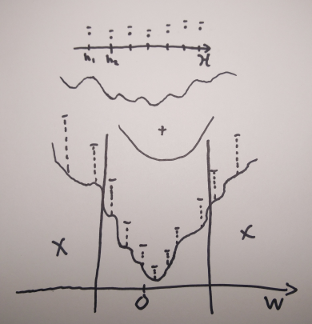
\includegraphics[scale=0.9,center]{schema.png}
	\newcommand{\seed}{1}
	\centering
    \begin{tikzpicture}[x=10pt,y=10pt,baseline,line cap=round]
        \pgfmathsetseed{\seed}
        \begin{scope}[thick]
            \draw[->] (-6,0) -- (6,0) node[below] {$w$};
            \draw[->] (0,-0.5) -- (0,6) node[right] {$R[h]$};
        \end{scope}
        \coordinate(p) at (-5,3);
        \foreach \i in {1,...,20}{
            \coordinate [at=(p), name=p\i];
            \coordinate(p) at ($(p)+(0.5,rand)$);
        }
        \draw[black!100] plot [smooth] coordinates {(p1) (p2) (p3) (p4) (p5) (p6) (p7) (p8) (p9) (p10) (p11) (p12) (p13) (p14) (p15) (p16) (p17) (p18) (p19) (p20)};
    \end{tikzpicture}
    +
    \begin{tikzpicture}[x=10pt,y=10pt,baseline,line cap=round]
        \pgfmathsetseed{\seed}
        \begin{scope}[thick]
            \draw[->] (-6,0) -- (6,0) node[below] {$w$};
            \draw[->] (0,-0.5) -- (0,6) node[right] {$R[h]$};
        \end{scope}
        \coordinate(p) at (-5,3);
        \foreach \i in {1,...,20}{
            \coordinate [at=(p), name=p\i];
            \coordinate(p) at ($(p)+(0.5,0)$);
            \pgfmathparse{(\i-10)/15}
            \coordinate(p) at ($(p)+(0,\pgfmathresult)$);
        }
        \draw[black!100] plot [smooth] coordinates {(p1) (p2) (p3) (p4) (p5) (p6) (p7) (p8) (p9) (p10) (p11) (p12) (p13) (p14) (p15) (p16) (p17) (p18) (p19) (p20)};
    \end{tikzpicture}
    =
    \begin{tikzpicture}[x=10pt,y=10pt,baseline,line cap=round]
        \pgfmathsetseed{\seed}
        \begin{scope}[thick]
            \draw[->] (-6,0) -- (6,0) node[below] {$w$};
            \draw[->] (0,-0.5) -- (0,6) node[right] {$R[h]$};
        \end{scope}
        \coordinate(p) at (-5,6);
        \foreach \i in {1,...,20}{
            \coordinate [at=(p), name=p\i];
            \coordinate(p) at ($(p)+(0.5,rand)$);
            \pgfmathparse{(\i-10)/15}
            \coordinate(p) at ($(p)+(0,\pgfmathresult)$);
        }
        \draw[black!100] plot [smooth] coordinates {(p1) (p2) (p3) (p4) (p5) (p6) (p7) (p8) (p9) (p10) (p11) (p12) (p13) (p14) (p15) (p16) (p17) (p18) (p19) (p20)};
    \end{tikzpicture}
    \caption{When an $\ell_2$ regularization term is added to the learning algorithm, it adds concavity to the loss function, leading to a higher likelihood of choosing a set of weights near the origin. In such a situation, using a prior which places heavier ``bets'' near the origin makes sense. This figure is a visual representation of what this loss function looks like after the addition of a regularization term.}
\end{figure}

\vspace*{0.5cm}
\begin{figure}[H]
    \captionsetup{justification=centering}
	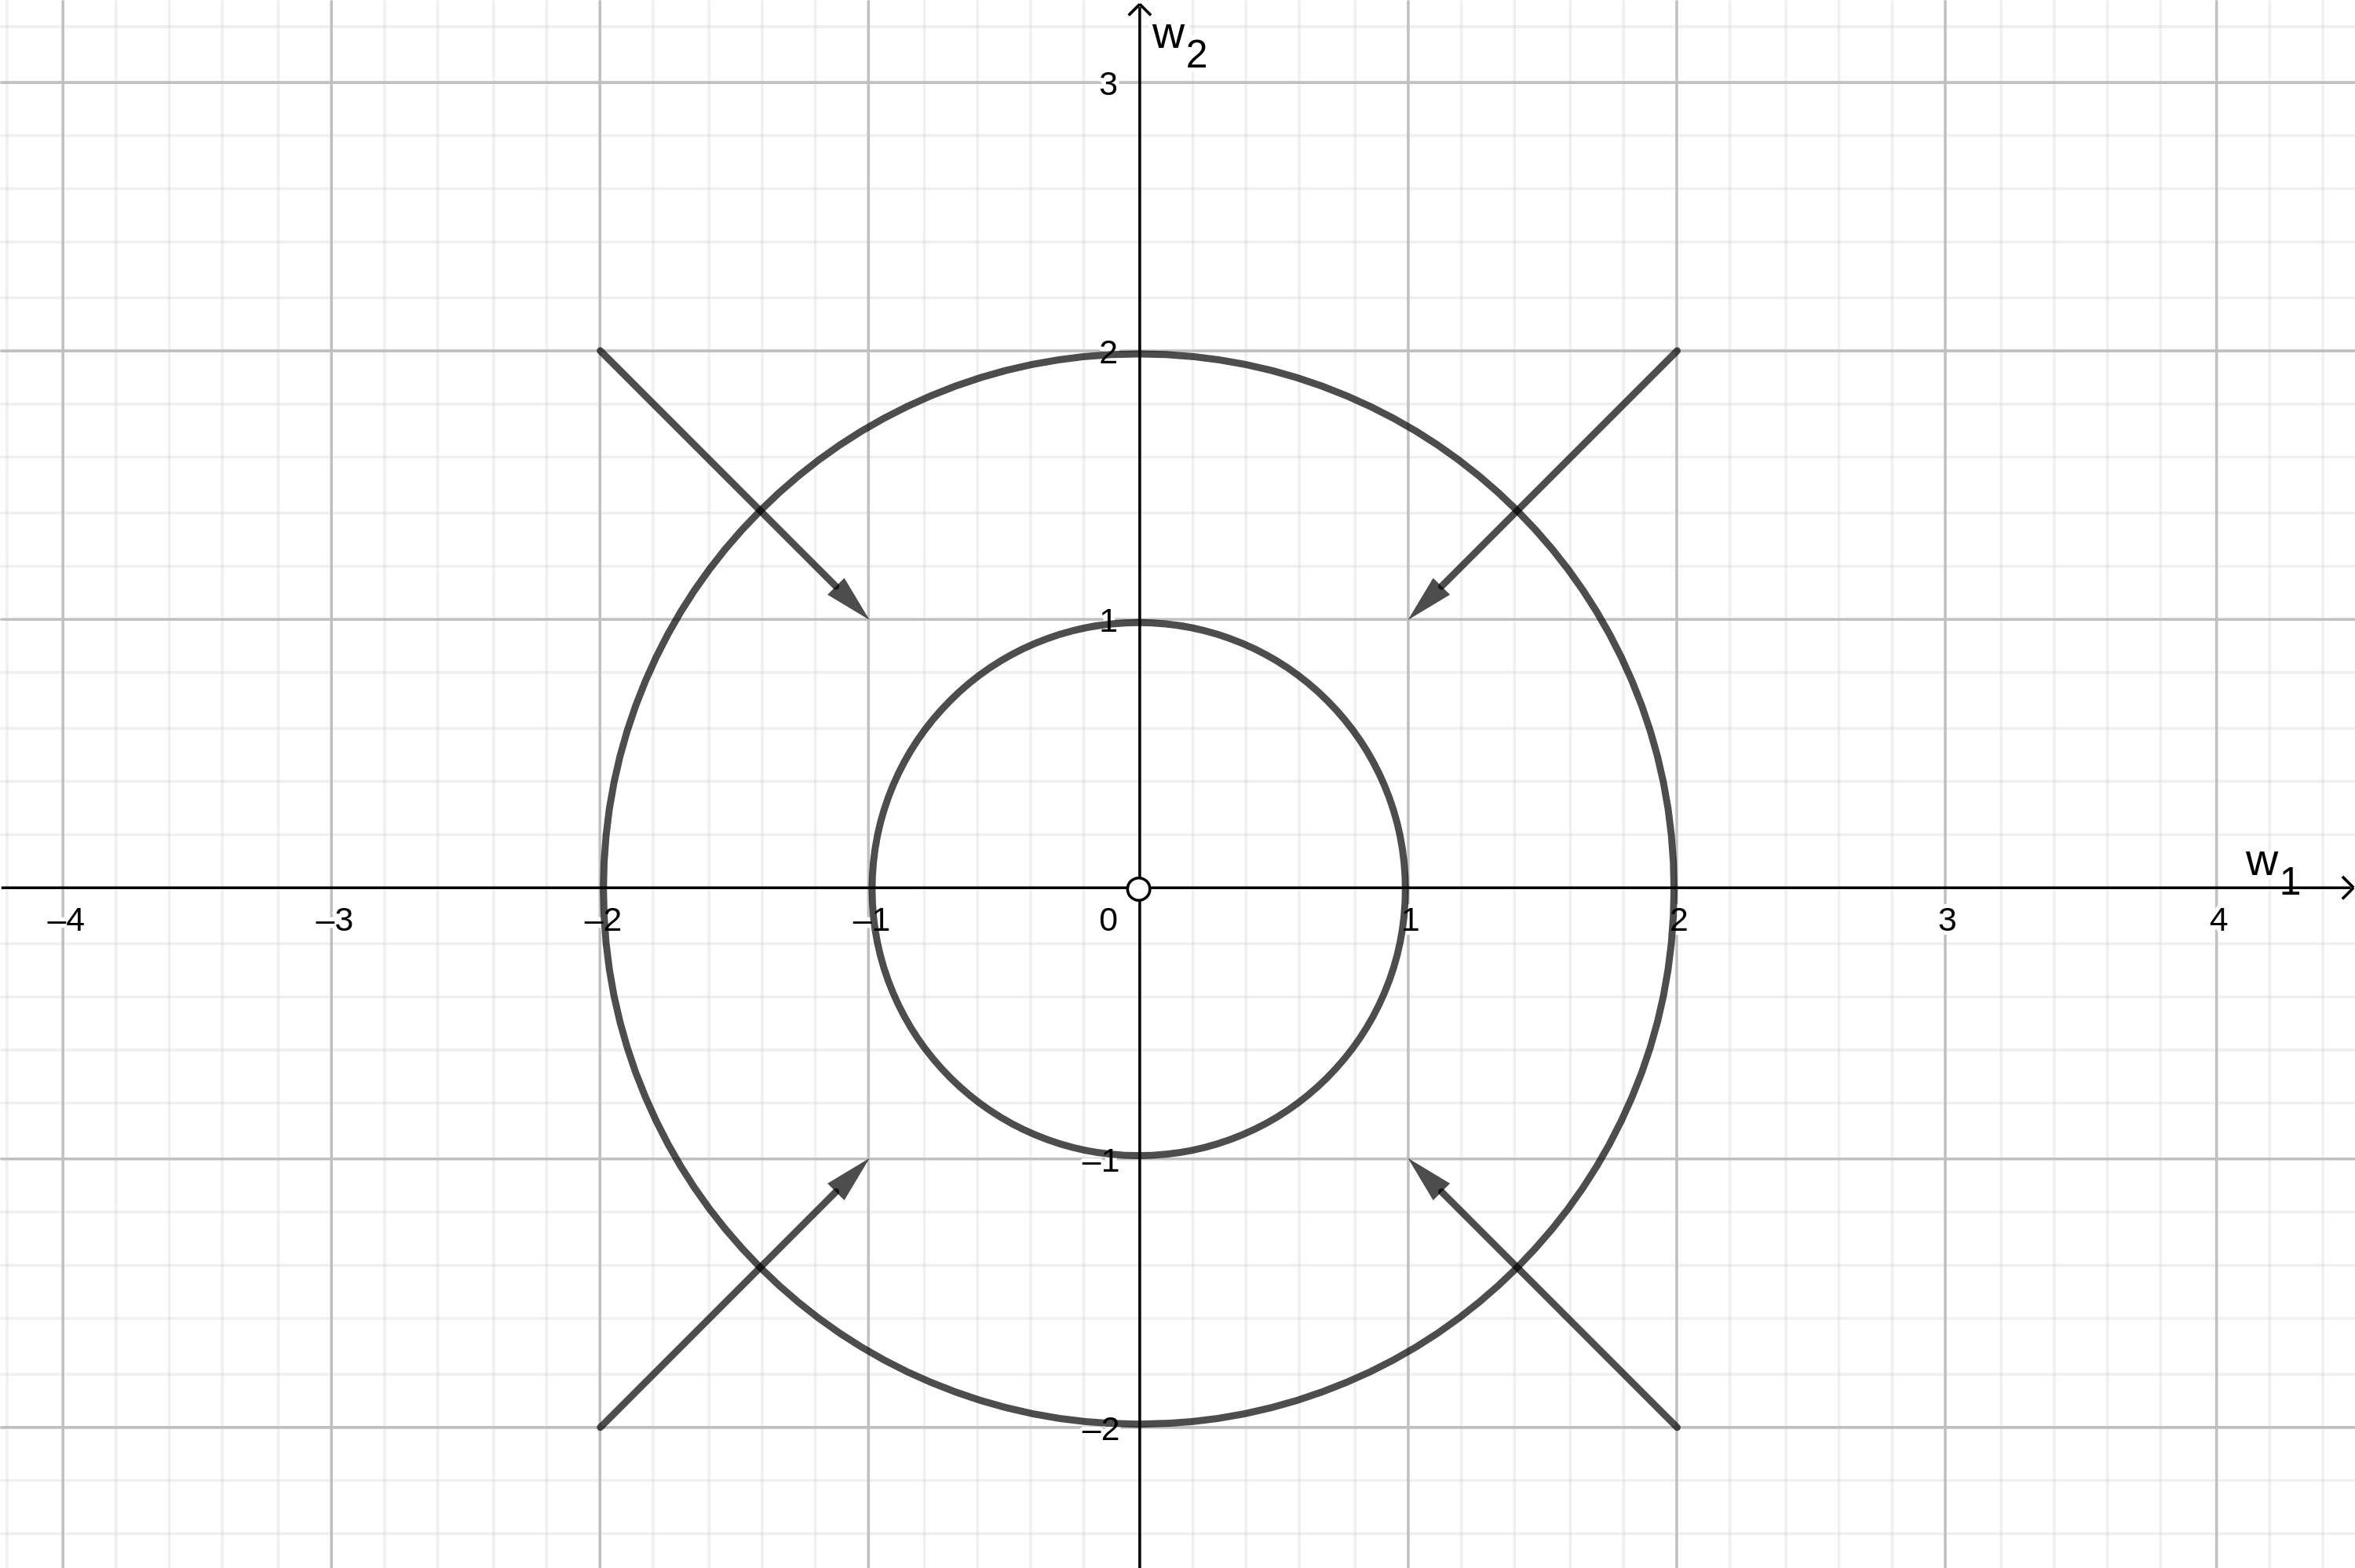
\includegraphics[scale=0.9,center]{circle.png}
    \caption{ \textbf{Example:} Consider a simple linear classifier with 2 weights $\Vec{w} = (w_1, w_2)$, which are stored using a 32 bit floats. This implies that the hypothesis class is finite with $|H|=2^{32 \times 2}$. Consider also that the loss function is bounded and has a \emph{regularization} term of the form $\lambda||\Vec{w}||$. The regularization term forces the weights to be as small as possible and corresponds to a prior $P$ with higher probability assigned to $\Vec{w}$ near the origin. In doing so we will get tight theoretical bounds for desirable hypotheses. Notice that this says nothing about the algorithm itself, we are just affecting how good our bounds are.}
\end{figure}

\section{PAC Bayes}
In PAC Bayes the basic idea is that we add a ``posterior'' $Q$ on $\mathcal{H}$, in addition to the prior $P$ we already had in the Occam's Bound. The basic recipe we follow is:
\begin{enumerate}
    \item Set our ``bets'' using the prior, $P$, independent of the data.
    \item We then collect some finite dataset $S\sim D$.
    \item Select a posterior, $Q$, based on the data.
\end{enumerate}
If we select the $Q=P$ as the posterior, then we get the same trade-off as in Occam's bound, wherein we get tight bounds on certain hypotheses, but not necessarily those we care about.
With the addition of this posterior, we can derive a new bound on the generalization gap that depends on the KL-divergence between the prior and the posterior:

\begin{thm}[PAC Bayes bound]
Given a prior probability distribution P over a hypothesis class H and a posterior probability distribution Q over H. Then: 
\[
	\mathbb{E}_{h \sim Q}[R[h]] \leq \mathbb{E}_{h \sim Q} [\hat{R_S}[h]] + \sqrt{\frac{D(Q||P) +
	\log(\frac{n}{\delta})}{2(n-1)}}
\] 
with probability $\geq 1 - \delta$.
\label{pacbayesbound}
\end{thm}
where 
\begin{defn}[Kullback-Leibler Divergence] The Kullback-Leibler (KL) divergence between two distributions Q and P is defined as:
\[
	D(Q||P) = \mathbb{E}_{h \sim Q}\bigg[\log\frac{Q(h)}{P(h)}\bigg]
\]
\end{defn}
is a measure of how far two probability distributions are\footnote{The KL-divergence is not symmetric - $D(Q||P) \neq D(P||Q)$ - and therefore is not a metric. Also note that $ P = Q \iff D(P||Q) = 0 $.}. In Theorem~\ref{pacbayesbound}, the KL-divergence serves as a complexity measure.

\begin{proof}
(See Theorem 31.1 of \cite{Shalev2014})
Recall the Markov inequality states that $P(X\geq a) \leq \frac{\mathbb{E}(X)}{a}$, and we can apply this to a function $f(S)$ to get
\begin{equation}
\mathbb{P}_S(f(S)\geq \epsilon) = \mathbb{P}_S(e^{f(S)} \geq e^\epsilon) \leq \frac{\mathbb{E}_S[e^{f(s)}]}{e^\epsilon}
\label{eqn:markov}
\end{equation}
Let $\Delta(h) = \mathbb{E}_{h\sim Q}[R[h]] - \mathbb{E}_{h\sim Q}[\hat R_S[h]]$.
We will apply equation (\ref{eqn:markov}) with the function
\[f(S) = \sup_Q \left(2(n-1)\mathbb{E}_{h\sim Q}(\Delta(h))^2 - D(Q||P)\right)\]
We now bound $\mathbb{E}_S[e^{f(S)}]$.
\begin{align*}
2(n-1)\mathbb{E}_{h\sim Q}(\Delta(h))^2 - D(Q||P)
&= \mathbb{E}_{h\sim Q} \left[\log(e^{2(n-1)\Delta(h)^2}P(h)/Q(h))\right]\\
\intertext{Apply Jensen's inequality, which tells us that $\mathbb{E}[\log(\cdot)]\leq \log\mathbb{E}(\cdot)$}
&\leq \log\mathbb{E}_{h\sim Q} \left[e^{2(n-1)\Delta(h)^2}P(h)/Q(h)\right]\\
\intertext{Use a ``twist of measures'' trick: $\mathbb{E}_{h\sim Q}[(\cdots) P(h)/Q(h)] = \sum_{h\in Q} Q(h)[(\cdots) P(h)/Q(h)] = \sum_{h\in Q}[(\cdots) P(h)] = \sum_{h\in P}[(\cdots) P(h)] = \mathbb{E}_{h\in P}[\cdots]$. }
&= \log\mathbb{E}_{h\sim P} \left[e^{2(n-1)\Delta(h)^2}\right]
\end{align*}
Therefore
\[\mathbb{E}_S[e^{f(S)}] \leq \mathbb{E}_S\mathbb{E}_{h\sim P}[e^{2(n-1)\Delta(h)^2}]\]
Since $P$ does not depend on $S$, we can swap the expectations
\begin{equation}
\mathbb{E}_S[e^{f(S)}] \leq \mathbb{E}_{h\sim P}\mathbb{E}_S[e^{2(n-1)\Delta(h)^2}]
\label{eqn:31.4}
\end{equation}
Next, we claim that for all $h$, we have $\mathbb{E}_S[e^{2(n-1)\Delta(h)^2}] \leq n$.
Recall that Hoeffding's inequality tells us that
\[\mathbb{P}_S[\Delta(h) \geq \epsilon] \leq e^{-2n\epsilon^2}\]
This implies that $\mathbb{E}_S[e^{2(n-1)\Delta(h)^2} \leq n]$.
Combining this with equation (\ref{eqn:31.4}) and plugging into equation (\ref{eqn:markov}), we get
\[\mathbb{P}_S[f(S) \geq \epsilon] \leq \frac{n}{e^\epsilon}\]
With $\delta=n/e^\epsilon$, we get $\epsilon=\log(n/\delta)$, and we obtain that with probability at least $1-\delta$ and for all $Q$,
\[2(n-1)\mathbb{E}_{h\sim Q} (\Delta(h))^2 - D(Q||P) \leq \epsilon = \log(n/\delta)\]
Rearranging the inequality and using Jensen's inequality again, we conclude that
\[\left(\mathbb{E}_{h\sim Q}\Delta(h)\right)^2 \leq \mathbb{E}_{h\sim Q}(\Delta(h))^2 \leq \frac{\log(n/\delta) + D(Q||P)}{2(n-1)}\]
\end{proof}

If we update our distribution over hypotheses using the posterior, $Q$, so that $h$ performs well on the empirical risk, it ensures that we can reduce $\mathbb{E}_{h\sim Q}[\hat{R_S}[h]]$ more than if we just sampled from the prior. However, we need to be careful of the complexity term that bounds our generalization on the true data distribution. If we choose a ``good'' posterior that is close to the prior, then the KL-divergence will become smaller and our bound will be tighter. 

Here are some examples of posteriors:
\begin{enumerate}
    \item Q assigns $h_S$ a probability of 1, i.e. $\mathbb{E}_{h\sim Q}[h] = h_S$. This means that $D(Q||P)\rightarrow \infty$ and the bound explodes (assuming $Q \neq P$).
    \item The posterior and the prior are the same, $Q=P$. This means that $D(Q||P)=0$ and the bound becomes tight. Even though this bound is tight, it is tight for hypotheses we may not care about, i.e. $\mathbb{E}_{h\sim P}[\hat{R_S}[h]]$ can be large.
    % TODO: Put this back when Ioannis talks more abbut it.
    % \item Let $Q=\mathcal{N}(h_S, I)$, that is \textcolor{red}{some interpretation about what this represents. since it has the same expectation as the 1st entry} $KL(Q||P)$ is finite and therefore, we can find bounds for $R_S[h]$. For example, if $R_s[h]$ is convex around $h$, Jensen's inequality will give $R[h]\leq \mathbb{E}_{h\sim Q}[R[h]]$.
\end{enumerate}


\vspace{0.5cm}
\bibliography{Refs/lec8}
\bibliographystyle{abbrvnat}


\end{document}